\documentclass[11pt]{article}
\usepackage[T1]{fontenc}
\usepackage{lmodern}
\usepackage[margin=1in]{geometry}
\usepackage{amsmath,amssymb,amsthm,mathtools}
\usepackage{graphicx,booktabs,longtable,array,enumitem,microtype,xurl}
\usepackage[hidelinks]{hyperref}
\usepackage{fancyhdr}
\setlength{\headheight}{14pt}
\pagestyle{fancy}
\fancyhf{}
\fancyhead[L]{\small Leading-index-one double polylogarithms}
\fancyhead[R]{\small ProveIt research continuation}
\fancyfoot[C]{\thepage}
\setlength{\parskip}{3pt}
\setlength{\parindent}{15pt}
\emergencystretch=2em
\numberwithin{equation}{section}
\newtheorem{theorem}{Theorem}[section]
\newtheorem{lemma}[theorem]{Lemma}
\newtheorem{proposition}[theorem]{Proposition}
\newtheorem{corollary}[theorem]{Corollary}
\theoremstyle{definition}
\newtheorem{definition}[theorem]{Definition}
\newtheorem{example}[theorem]{Example}
\theoremstyle{remark}
\newtheorem{remark}[theorem]{Remark}
\DeclareMathOperator{\Li}{Li}
\DeclareMathOperator{\Imn}{Im}
\DeclareMathOperator{\Ren}{Re}
\DeclareMathOperator{\atanh}{atanh}
\newcommand{\dd}{\,\mathrm d}
\newcommand{\ii}{\mathrm i}
\newcommand{\C}{\mathbb C}
\newcommand{\R}{\mathbb R}
\newcommand{\E}{\mathbb E}
\newcommand{\cut}{\C\setminus[1,\infty)}
\newcommand{\Qw}{Q_w}
\newcommand{\Wtot}{\mathsf W}
\newcommand{\src}[1]{\nolinkurl{#1}}
\newcommand{\repocommit}{\texttt{1539f353af88bdfd63292bb970ac8f585b15794d}}
\hypersetup{pdftitle={Global radial monotonicity for leading-index-one double polylogarithms},pdfauthor={OpenAI ChatGPT, prepared for the ProveIt research program}}

\begin{document}
\begin{titlepage}
\thispagestyle{empty}
\vspace*{0.3in}
{\large\sffamily PROVEIT\quad /\quad ANALYSIS\quad /\quad POLYLOGARITHMS\par}
\vspace{0.45in}
{\LARGE\bfseries Global Radial Monotonicity for\\[5pt]
Leading-Index-One Double Polylogarithms\par}
\vspace{0.22in}
{\Large Reflected Green curvature, Cauchy-mode flow,\\
odd-moment inequalities, and exact weight-generating identities\par}
\vspace{0.35in}
{\large Prepared by OpenAI ChatGPT for Vladimir Reshetnikov's\\
ProveIt research program\par}
\vspace{0.12in}
{10 October 2026\par}
\vspace{0.3in}
\begin{abstract}
For every real $b>0$, let $\theta_{1,b}(\rho)$ be the unique zero of
$\Imn\Li_{1,b}(\rho e^{\ii\theta},1)$ on the upper semicircle of radius
$0<\rho\le1$. We prove the complete leading-index-one part of the
normalized-radius conjecture stated in the inspected ProveIt manuscript:
$\eta_{1,b}(\rho)=\cos\theta_{1,b}(\rho)/\rho$ is strictly decreasing for
$b>1$, strictly increasing for $0<b<1$, and identically $1/2$ for $b=1$.
The proof is global in radius, not a Taylor-series sign argument.

A Dirichlet Green transform converts the polylogarithm into a second-order
Stieltjes integral with a strictly concave positive density. In inverse
coordinates, its imaginary-part zero is exactly the mode of a
Cauchy-smoothed density. A reflected-curvature criterion proves strict
motion of that mode, and a separate implicit derivative converts it to
the required radial sign. The criterion applies more generally to
Student-type kernels and to two monotone sectors of Hurwitz-shifted inner
orders. It also proves the sign of every odd central moment of an explicit
harmonic-moment probability law.

We obtain an exact upper-half-plane parametrization, an all-circle cutoff
for $b\ge1$, a two-term radial correction, and opposite radial-curvature
signs at $b=2$ and $b=4$. An independent weight-generating identity yields
closed sums over every odd and every even inner order, including sums
at $z=-1$ and $z=1/4$. The package contains self-contained proofs,
18 rational root certificates, 1,938 exact finite regression checks,
five symbolic checks, numerical diagnostics, and an additive manuscript
fragment. The arguments do not resolve the remaining higher-outer-order
radial problem or the S6 and S8 arithmetic candidates.
\end{abstract}
\vfill
\noindent\textbf{Status.} Research manuscript with ordinary mathematical proofs;
not independently peer reviewed or proof-assistant formalized. The claimed
advance is relative to the explicitly inspected source section. No claim
of worldwide priority, exhaustive repository audit, or inspection of all
incoming archive contents is made.
\end{titlepage}

\begingroup
\small
\setlength{\parskip}{0pt}
\tableofcontents
\endgroup
\newpage

\section{The question and the precise advance}
\label{sec:intro}
For $b>0$, write
\begin{equation}\label{eq:Fdef}
 F_b(z)=F_{1,b}(z)=\Li_{1,b}(z,1)
 =\sum_{n=2}^{\infty}\frac{H_{n-1}^{(b)}}n z^n,
 \qquad H_N^{(b)}=\sum_{k=1}^N k^{-b}.
\end{equation}
Initially $|z|<1$; throughout the paper the continuation is the one on
$\cut$ that agrees with this series. The ordinary depth-one polylogarithm
and logarithm use the conventions of DLMF~25.12~\cite{dlmf}.
A ``zero'' of an angular imaginary part is not a zero of the complex
function itself.

The ProveIt chapter fragment
\src{chapters/05-real-local-radius.tex} states a normalized-radius
conjecture and proves the sign of its first nonconstant local
coefficient~\cite{repo-local}. At leading index one it predicts exactly
the three cases in the next theorem. The general signed-kernel chapter
already establishes uniqueness and simplicity of the relevant angular
zero~\cite{repo-signed}. We reprove the portion needed here to make all
subsequent sign arguments self-contained.

\begin{theorem}[Complete leading-index-one radial law]\label{thm:main}
For every $b>0$ and $0<\rho\le1$ there is exactly one
$\theta_{1,b}(\rho)\in(0,\pi)$ such that
\[
 \Imn F_b(\rho e^{\ii\theta_{1,b}(\rho)})=0.
\]
Set $\eta_b(\rho)=\cos\theta_{1,b}(\rho)/\rho$. Then
\begin{equation}\label{eq:main-sign}
 \eta_b'(\rho)
 \begin{cases}
 <0,&b>1,\\
 =0,&b=1,\\
 >0,&0<b<1.
 \end{cases}
 \qquad \eta_1(\rho)=\frac12.
\end{equation}
The function extends real analytically as an even function near zero,
with
\begin{equation}\label{eq:meanb}
 \eta_b(0)=\mu_b:=\frac{1+2^{-b}}3.
\end{equation}
Let $r_b$ be the unique maximum point of the density $Q_b$ in
\eqref{eq:Qb}. For all positive disk radii,
\begin{align}
 0<r_b<\eta_b(\rho)<\mu_b<\tfrac12,
       && b>1,\label{eq:boundsbhigh}\\
 \tfrac12<\mu_b<\eta_b(\rho)<r_b<1,
       && 0<b<1.\label{eq:boundsblow}
\end{align}
At $\rho=1$, the derivative means the derivative of the local analytic
continuation of the same simple root; in particular the corresponding
one-sided derivative has the displayed sign.
\end{theorem}

The proof occupies Sections~\ref{sec:green}--\ref{sec:radial}. Its main
new mechanism is an ordered sign change of a reflected density. Mere
unimodality is not sufficient to infer the direction of motion of a mode;
and motion in inverse height does not, by itself, imply motion in disk
radius. These two additional steps are proved explicitly.

\subsection{Additional results and boundaries of the claim}
The same method proves a mode-flow theorem for a class of Green densities
and every kernel $((x-u)^2+y^2)^{-\alpha}$, $\alpha>0$.
It gives the whole imaginary-zero curve in the upper half-plane, including
a finite-radius cutoff when $b\ge1$. A probability measure with raw
moments $2H_{j+1}^{(b)}/((j+1)(j+2))$ has all nontrivial odd central
moments of the sign of $b-1$. The manuscript's local coefficient is
exactly minus twice its third central moment. Nevertheless, the next
radial coefficient changes sign: monotonicity does not entail a universal
curvature sign.

A separate exact generating function sums over the inner order. Its
half-integer specializations give
\begin{align}
 \sum_{j\ge0}4^{-j}F_{2j+1}(-1)&=\frac\pi2-\frac{\pi^2}{8},
       \label{eq:introodd}\\
 \sum_{j\ge0}4^{-j}F_{2j+2}(-1)&=\pi-4\log2.
       \label{eq:introeven}
\end{align}
These are proved identities, not integer-relation guesses. Their
functional versions hold on the principal slit plane.

Nothing here proves the complete normalized-radius assertion at larger
outer orders. In particular, this paper does not promote the S6 or S8
period relations from numerically supported candidates to theorems.
The source README expressly keeps those relations conjectural~\cite{repo-readme}.
The distinction is important: the present advance is an analytic
monotonicity theorem, not a finite-basis reduction of those constants.

\subsection{Literature and source scope}
Ibragimov's strong-unimodality theorem relates log-concavity to preservation
of unimodality under convolution~\cite{ibragimov}. Our proof of unique
smoothed modes uses that classical mechanism and supplies the strict
second-derivative statement needed for differentiation. We do not claim
strong unimodality itself as a new result. Hausdorff moment generating
functions and their Pick-function structure provide related background
in Liu--Pego~\cite{liu-pego}; the consulted arXiv version includes their
2025 corrigendum. Neither external theorem is used as an unproved step
in the radial argument.

The source pin is the ProveIt commit
\begin{center}\repocommit.\end{center}
The local-radius fragment was re-read at that exact pin and has blob
\src{30e3e31944be5bc0d03a8485386dd1608c075507}.
The manuscript README, relevant analytic fragments, and incoming intake
README and directory listing were also inspected. The incoming ZIP
members were not available for content-level inspection in this session.
Accordingly, novelty is assessed against the named manuscript statements,
not against an asserted exhaustive inventory of all incoming results.

\section{A Green transform with harmonic moments}
\label{sec:green}
\subsection{The general density and its endpoint control}
\begin{definition}\label{def:w}
An admissible weight is a continuous positive function
$w:(0,1)\to(0,\infty)$ with
$\Wtot=\int_0^1w(t)\dd t<\infty$. Define
\begin{equation}\label{eq:Qgeneral}
 \Qw(u)=(1-u)\int_0^u\frac{w(t)}{1-t}\dd t
             +u\int_u^1\frac{w(t)}t\dd t,\qquad 0<u<1.
\end{equation}
Set $\Qw(0)=\Qw(1)=0$, and extend it by zero outside $[0,1]$ whenever
it occurs in a convolution or reflection.
\end{definition}

The factors outside the integrals in \eqref{eq:Qgeneral} are essential.
The separate endpoint integrals can be infinite at $u=0$ or $u=1$,
but their displayed products have well-defined limits. This point
matters for every $0<b<1$ in the polylogarithm application.

\begin{lemma}[Green regularity and exact moments]\label{lem:green}
For every admissible $w$, $\Qw$ is continuous on $[0,1]$, absolutely
continuous there, strictly positive on $(0,1)$, and strictly concave.
It is twice continuously differentiable in the open interval and
\begin{align}
 \Qw'(u)&=\int_u^1\frac{w(t)}t\dd t
                    -\int_0^u\frac{w(t)}{1-t}\dd t,
                    \label{eq:Qprime}\\
 \Qw''(u)&=-\frac{w(u)}{u(1-u)}<0.\label{eq:curvature}
\end{align}
Its logarithm is strictly concave on $(0,1)$. Moreover,
\begin{equation}\label{eq:Qmoments}
 \int_0^1u^j\Qw(u)\dd u
 =\frac1{(j+1)(j+2)}
   \int_0^1 w(t)\frac{1-t^{j+1}}{1-t}\dd t,
 \qquad j\ge0.
\end{equation}
In particular its mass is $\Wtot/2$.
\end{lemma}
\begin{proof}
Write $G(u,t)=\min(u,t)(1-\max(u,t))$. Then
\[
 \Qw(u)=\int_0^1\frac{G(u,t)}{t(1-t)}w(t)\dd t.
\]
The ratio in this integrand is between zero and one, and tends to zero
as $u$ tends to either endpoint, for each fixed $t\in(0,1)$.
Dominated convergence proves continuity and the two zero limits, and
also gives $\Qw\le\Wtot$. Positivity is immediate.

Differentiating in the open interval gives \eqref{eq:Qprime} and
\eqref{eq:curvature}. The two positive terms in \eqref{eq:Qprime} each
have integral $\Wtot$ over $u\in(0,1)$, by Tonelli. Thus
$\Qw'\in L^1(0,1)$, and the interior fundamental theorem of calculus
extends to both endpoints. Strict concavity follows from
\eqref{eq:curvature}; strict log-concavity follows from
\[
 (\log\Qw)''=\frac{\Qw''}{\Qw}
                        -\left(\frac{\Qw'}{\Qw}\right)^2<0.
\]
Finally, a direct integration of the two linear pieces of $G$ gives
\[
 \int_0^1u^jG(u,t)\dd u
       =\frac{t-t^{j+2}}{(j+1)(j+2)}.
\]
Tonelli now proves \eqref{eq:Qmoments}. This derivation does not assume
that either unweighted endpoint integral in \eqref{eq:Qprime} is finite.
\end{proof}

\subsection{A signed measure and a second-order Stieltjes integral}
Put $\kappa_w=-\Qw'$. It is integrable, strictly increasing, and has
zero integral. It therefore has a unique strict negative-to-positive
crossing $r_w\in(0,1)$, which is the unique maximum point of $\Qw$.
Define
\begin{equation}\label{eq:Fw}
 \mathcal F_w(z)=z\int_0^1\frac{\kappa_w(u)}{1-zu}\dd u
             =z^2\int_0^1\frac{\Qw(u)}{(1-zu)^2}\dd u.
\end{equation}
Integration by parts proves the equality; absolute continuity and
$\Qw(0)=\Qw(1)=0$ remove the boundary terms. Both integrals are
holomorphic on $\cut$. Indeed, on a compact subset of this domain,
$|1-zu|$ has a uniform positive lower bound for $0\le u\le1$.

The moments in Lemma~\ref{lem:green} give the disk series
\begin{equation}\label{eq:Fwcoeff}
 \mathcal F_w(z)=\sum_{n\ge2}\frac{z^n}{n}
    \int_0^1w(t)\frac{1-t^{n-1}}{1-t}\dd t.
\end{equation}
They also show, directly, that
\[
 \int_0^1u^{n-1}\kappa_w(u)\dd u
       =(n-1)\int_0^1u^{n-2}\Qw(u)\dd u
\]
for $n\ge2$, while the $n=1$ moment is zero.

\begin{remark}[A positive first-order transform after a factor]
The one-crossing property also gives
\begin{equation}\label{eq:nonvanishing}
 \mathcal F_w(z)=\frac{z^2}{1-r_wz}
  \int_0^1\frac{(u-r_w)\kappa_w(u)}{1-zu}\dd u.
\end{equation}
The new numerator is positive except at its crossing. The integral is
positive for real $z<1$ and has the sign of $\Imn z$ in its imaginary
part off the real axis. Thus $\mathcal F_w$ has no nonzero zeros in
the slit plane. This is a useful direct check that the curves studied
below concern imaginary parts, not complex zeros. Comparable
nonvanishing results already occur in the source manuscript; the new
contribution is their radial geometry.
\end{remark}

\subsection{Specialization to inner polylogarithm order}
Take
\begin{equation}\label{eq:wb}
 w_b(u)=\frac{(-\log u)^{b-1}}{\Gamma(b)},\qquad b>0.
\end{equation}
The gamma integral gives
\[
 \int_0^1u^k w_b(u)\dd u=(k+1)^{-b},\qquad k\ge0.
\]
Consequently $\Wtot=1$, \eqref{eq:Fwcoeff} becomes \eqref{eq:Fdef},
and the associated Green density has the explicit form
\begin{equation}\label{eq:Qb}
 Q_b(u)=\frac{u(-\log u)^b}{\Gamma(b+1)}
 +\frac{1-u}{\Gamma(b)}
       \int_0^u\frac{(-\log t)^{b-1}}{1-t}\dd t.
\end{equation}
The probability density $2Q_b$ therefore has moments
\begin{equation}\label{eq:rawb}
 \E U_b^j=\frac{2H_{j+1}^{(b)}}{(j+1)(j+2)},\qquad j\ge0,
\end{equation}
and mean $\mu_b$ from \eqref{eq:meanb}. Its curvature is
\begin{equation}\label{eq:Qbcurvature}
 -u(1-u)Q_b''(u)=w_b(u).
\end{equation}
The right side is strictly decreasing when $b>1$, strictly increasing
when $0<b<1$, and constant when $b=1$. This elementary observation
will control a global zero curve.

For $b=1$,
\begin{equation}\label{eq:entropy}
 Q_1(u)=-u\log u-(1-u)\log(1-u),\qquad
 F_1(z)=\tfrac12\log^2(1-z).
\end{equation}
For a positive integer $m$, the density also has a finite polylogarithmic
expression. With $T=-\log u$,
\begin{equation}\label{eq:Qinteger}
 Q_m(u)=\frac{uT^m}{m!}
 +(1-u)\sum_{j=0}^{m-1}\frac{T^j}{j!}\Li_{m-j}(u).
\end{equation}
To prove this, substitute $t=e^{-v}$ in the integral of \eqref{eq:Qb},
expand $(e^v-1)^{-1}$ as a positive exponential series, and integrate
$v^{m-1}e^{-kv}$ from $T$ to infinity. Its finite incomplete-gamma
formula gives exactly the displayed sum.

\section{Unique modes under Cauchy and Student-type smoothing}
\label{sec:modes}
For $\alpha>0$, $y>0$, define
\begin{equation}\label{eq:A}
 A_{\alpha,y}(x)=\int_0^1
        \frac{\Qw(u)}{((x-u)^2+y^2)^\alpha}\dd u.
\end{equation}
The kernel is integrable on the whole line only when $\alpha>1/2$,
but \eqref{eq:A} is finite and analytic for every $\alpha>0$ because
$\Qw$ has compact support. Thus ``Student-type'' here describes the
kernel shape, not a claim of probability normalization for every
$\alpha$.

\begin{lemma}[Strict unique mode]\label{lem:mode}
For every admissible $w$, every $\alpha>0$, and every $y>0$,
$A_{\alpha,y}$ has exactly one stationary point
$m_\alpha(y)\in(0,1)$. It is a strict maximum and
\begin{equation}\label{eq:nondegenerate}
 \partial_x^2A_{\alpha,y}(m_\alpha(y))<0.
\end{equation}
The function $m_\alpha$ is real analytic on $(0,\infty)$.
\end{lemma}
\begin{proof}
Let $K(v)=(v^2+y^2)^{-\alpha}$. Then $K'(v)$ is positive for $v<0$
and negative for $v>0$. Therefore $A_x(x)>0$ for $x\le0$ and
$A_x(x)<0$ for $x\ge1$, so at least one stationary point lies between.

Fix any such point $x$. After $v=x-u$, the stationary equation is
\[
 \int_{x-1}^{x}\Qw(x-v)K'(v)\dd v=0.
\]
The signed integrand is positive on $v<0$ and negative on $v>0$.
The logarithmic score
\[
 S(v)=\frac{\Qw'(x-v)}{\Qw(x-v)}
\]
is strictly increasing, since $(\log\Qw)''<0$. Using the zero integral
and subtracting $S(0)$ gives
\begin{align*}
 A_{xx}(x)
 &=\int_{x-1}^{x}\Qw'(x-v)K'(v)\dd v\\
 &=\int_{x-1}^{x}\Qw(x-v)K'(v)(S(v)-S(0))\dd v<0.
\end{align*}
The integration by parts implicit in the first equality is legitimate:
$\Qw$ vanishes at the endpoints, $\Qw'$ is integrable, and $K'$ is
bounded on the finite integration range. The score need not remain
bounded near the endpoints; the product is still integrable by this
same $L^1$ bound.

Thus every zero of $A_x$ crosses strictly from positive to negative.
There cannot be two such zeros, because between two downward crossings
a continuous derivative must return from negative to positive, forcing
a zero that is not a strict downward crossing. This proves uniqueness
and \eqref{eq:nondegenerate}. The analytic implicit-function theorem
applies to $A_x=0$, since the integral is locally real analytic in
$(x,y)$ for $y>0$.
\end{proof}

\begin{remark}[Which function is log-concave]
It is $\Qw$, not the Cauchy kernel, whose log-concavity is used.
The Cauchy kernel is not log-concave on the entire real line.
Lemma~\ref{lem:mode} is a strict, directly proved version of the
strong-unimodality mechanism associated with Ibragimov~\cite{ibragimov}.
It does not yet determine a direction for $m_\alpha'(y)$.
\end{remark}

\section{Reflected curvature and strict mode flow}
\label{sec:reflection}
The central step is a geometric consequence of the normalized curvature
$-u(1-u)\Qw''(u)=w(u)$.

\begin{lemma}[A reflected single crossing]\label{lem:reflection}
Suppose $w$ is nonconstant and nonincreasing. For $0<x<1/2$, put
\begin{equation}\label{eq:Delta}
 \Delta_x(v)=\Qw(x+v)-\Qw(x-v),\qquad v\ge0,
\end{equation}
using the zero extension. Then $\Delta_x$ is strictly convex on $(0,x)$,
$\Delta_x(0)=0$, and $\Delta_x(x)=\Qw(2x)>0$.
It is positive for $x\le v<1-x$ and zero for $v\ge1-x$.
If it takes a negative value, it has exactly one negative-to-positive
crossing $v_0\in(0,x)$ on its nonzero support.
At $x=1/2$, $\Delta_{1/2}(v)<0$ for $0<v<1/2$.
\end{lemma}
\begin{proof}
For $0<v<x<1/2$, \eqref{eq:curvature} gives
\begin{equation}\label{eq:Delta-curvature}
 \Delta_x''(v)=
 \frac{w(x-v)}{(x-v)(1-x+v)}
 -\frac{w(x+v)}{(x+v)(1-x-v)}>0.
\end{equation}
Indeed, the numerator in the first term is no smaller, whereas its
denominator is strictly smaller, because the difference of the two
denominators is $2v(1-2x)>0$. The support and endpoint statements
follow directly from the zero extension.

Strict convexity and $\Delta_x(0)=0$ imply that
$\Delta_x(v)/v$ is strictly increasing on $(0,x)$. Thus a negative value
and the positive value at $x$ force one and only one positive crossing
before $x$. Beyond $x$ the difference is already positive.

At $x=1/2$, the denominator difference vanishes and the numerator
ordering gives $\Delta''\ge0$. It is not identically zero: otherwise
$w(1/2-v)=w(1/2+v)$ for all $v$, and a nonincreasing symmetric function
would be constant. Since both endpoints of $\Delta$ are zero, convexity
and nonlinearity make $\Delta$ strictly negative in the open interval.
\end{proof}

\begin{theorem}[Monotone Green curvature forces monotone mode flow]
\label{thm:modeflow}
Let $w$ be admissible and $\alpha>0$. If $w$ is nonconstant and
nonincreasing, then
\begin{equation}\label{eq:modeflow-downw}
 0<m_\alpha(y)<\tfrac12,\qquad m_\alpha'(y)>0\quad(y>0).
\end{equation}
If $w$ is nonconstant and nondecreasing, then
\begin{equation}\label{eq:modeflow-upw}
 \tfrac12<m_\alpha(y)<1,\qquad m_\alpha'(y)<0\quad(y>0).
\end{equation}
If $w$ is constant, $m_\alpha(y)=1/2$ for all $y$.
\end{theorem}
\begin{proof}
First suppose $w$ is nonconstant and nonincreasing. Write $t=y^2$.
Pairing the two sides of $x$ in the derivative of \eqref{eq:A} gives
\begin{equation}\label{eq:Ialpha}
 A_x(x)=2\alpha I_\alpha(x,t),\qquad
 I_\alpha(x,t)=\int_0^\infty
    \frac{v\Delta_x(v)}{(v^2+t)^{\alpha+1}}\dd v.
\end{equation}
Lemma~\ref{lem:reflection} gives $A_x(1/2)<0$. By unique modehood,
the mode $x=m_\alpha(y)$ lies below $1/2$.

At this mode, $I_\alpha=0$. The positive part of $\Delta_x$ near and
beyond $v=x$ is nonempty, so the zero integral forces a negative part.
Lemma~\ref{lem:reflection} therefore gives a unique crossing $v_0$,
with negative sign before and positive sign after it. Differentiate
with respect to $t$ at fixed $x$ and subtract a constant multiple of
the zero integral:
\begin{align}\label{eq:It-sign}
 \partial_tI_\alpha(x,t)
 &=\int_0^\infty\frac{v\Delta_x(v)}{(v^2+t)^{\alpha+1}}
 \left(-\frac{\alpha+1}{v^2+t}
                +\frac{\alpha+1}{v_0^2+t}\right)\dd v>0.
\end{align}
The parenthesized factor is strictly increasing in $v>0$ and vanishes
at $v_0$; hence its sign agrees with that of $\Delta_x$.
All differentiations are dominated because $t>0$ and the support is
bounded.

By Lemma~\ref{lem:mode}, $I_{\alpha,x}<0$ at the root. Implicit
differentiation gives
\[
 \frac{d m_\alpha}{dt}=-\frac{I_{\alpha,t}}{I_{\alpha,x}}>0,
 \qquad m_\alpha'(y)=2y\frac{d m_\alpha}{dt}>0.
\]
For a nondecreasing weight, reflect $u\mapsto1-u$. Its Green density
is reflected as well, so every inequality reverses. A constant weight
has a symmetric density, whose unique mode is the center.
\end{proof}

\begin{figure}[tbp]
\centering
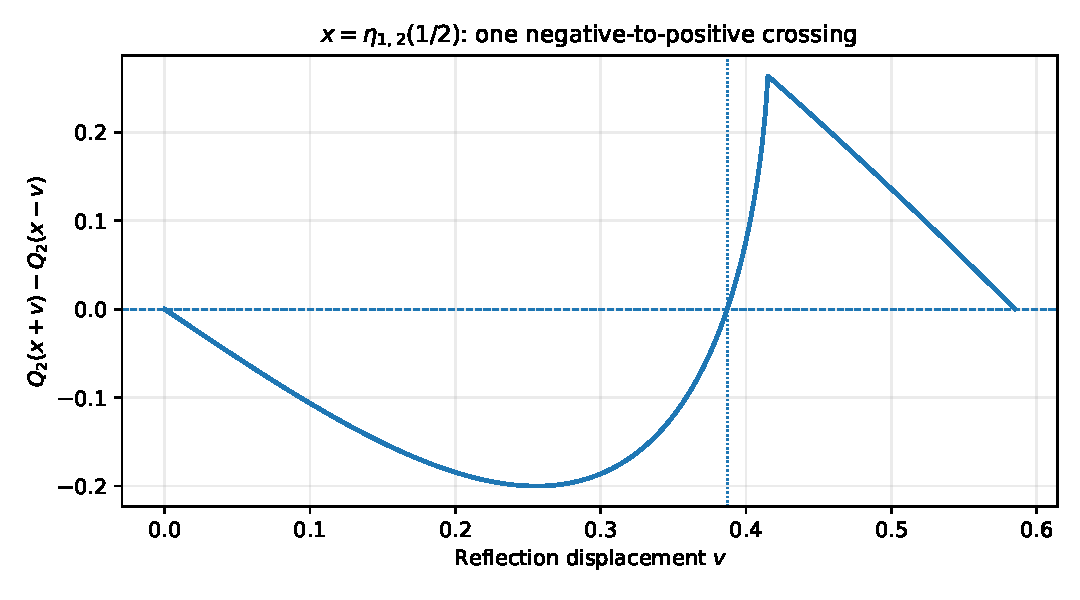
\includegraphics[width=0.94\linewidth]{figures/reflected_difference.pdf}
\caption{The decisive sign change, illustrated with $b=2$ and
$x=\eta_2(1/2)$. The graph is a floating-point illustration, not a
certificate. The unique negative-to-positive crossing is proved by
\eqref{eq:Delta-curvature}; the positive derivative in
\eqref{eq:It-sign} follows by weighting this same crossing.}
\label{fig:reflection}
\end{figure}

\subsection{The Cauchy mode interpolates between mode and mean}
For $\alpha=1$, multiplication by $y/\pi$ gives the usual Poisson,
or Cauchy, kernel
\[
 P_y(v)=\frac{y}{\pi(v^2+y^2)}.
\]
Write $m(y)=m_1(y)$ and let $\mu_w$ be the mean of the probability
density $2\Qw/\Wtot$. Formula~\eqref{eq:Qmoments} gives
\begin{equation}\label{eq:muw}
 \mu_w=\frac13\left(1+\frac{\int_0^1t w(t)\dd t}{\Wtot}\right).
\end{equation}

\begin{corollary}[Strict interpolation]\label{cor:interpolation}
For every admissible $w$,
\begin{equation}\label{eq:mode-limits}
 \lim_{y\downarrow0}m(y)=r_w,\qquad
 \lim_{y\to\infty}m(y)=\mu_w.
\end{equation}
If $w$ is nonconstant and nonincreasing, then
\[
 0<r_w<m(y)<\mu_w<\tfrac12.
\]
If it is nonconstant and nondecreasing, then
\[
 \tfrac12<\mu_w<m(y)<r_w<1.
\]
\end{corollary}
\begin{proof}
The zero extension of $\Qw$ is continuous and compactly supported.
Thus $P_y*\Qw\to\Qw$ uniformly as $y\downarrow0$, by the elementary
approximate-identity argument. Each maximum lies in $[0,1]$, and any
limit point of the maxima must maximize $\Qw$. Its strict concavity
leaves only $r_w$.

For large $y$, the stationary equation is
\[
 0=\int_0^1 (u-m(y))\Qw(u)
          \left(1+\frac{(u-m(y))^2}{y^2}\right)^{-2}\dd u.
\]
The factor in parentheses tends uniformly to one for $m(y)\in[0,1]$.
It follows that $m(y)\to\mu_w$.

Strict inequalities between the endpoint limits follow from
Theorem~\ref{thm:modeflow}. Finally, if $w$ is nonconstant and
nonincreasing, pairing $t$ and $1-t$ shows
$\int_0^1(t-1/2)w(t)\dd t<0$, so \eqref{eq:muw} gives
$\mu_w<1/2$. Reflection handles the other case.
\end{proof}

\section{From mode flow to the global radial theorem}
\label{sec:radial}
\subsection{The known angular root, with its derivative sign}
\begin{lemma}[Angular existence, uniqueness, and simplicity]
\label{lem:angular}
For every admissible $w$ and $0<\rho\le1$, the function
$\Imn\mathcal F_w(\rho e^{\ii\theta})$ has exactly one zero on
$0<\theta<\pi$. With $c=\cos\theta$, this root lies in $0<c<\rho$.
It is simple, and the imaginary part has a negative angular derivative
there.
\end{lemma}
\begin{proof}
Let $\kappa=\kappa_w$, and put
\begin{equation}\label{eq:J}
 J_\rho(c)=\int_0^1\frac{\kappa(u)}{1-2\rho cu+\rho^2u^2}\dd u.
\end{equation}
Then the imaginary part is $\rho\sin\theta\,J_\rho(c)$.
For any strictly increasing function $h$, subtraction of $h(r_w)$
shows $\int h\kappa>0$; for a strictly decreasing $h$ the sign is
negative. In particular, $J_\rho(0)<0$.
At $c=\rho$ the denominator's derivative in $u$ is
$-2\rho^2(1-u)<0$, so its reciprocal is strictly increasing and
$J_\rho(\rho)>0$. If $\rho=1$, this is interpreted as a positive,
possibly infinite, endpoint limit. The negative part of $\kappa$ is
away from the singular endpoint; the positive part is treated by
monotone convergence. No difference of divergent integrals is used.

Set $K_c(u)=(1-2\rho cu+\rho^2u^2)^{-1}$. For $c'>c$,
\begin{equation}\label{eq:kernelratio}
 \frac d{du}\frac{K_{c'}(u)}{K_c(u)}
 =\frac{2\rho(c'-c)(1-\rho^2u^2)}
              {(1-2\rho c'u+\rho^2u^2)^2}>0.
\end{equation}
At a zero $J_\rho(c)=0$, the signed measure $K_c\kappa\dd u$ has
zero mass and the same one-crossing sign pattern. The increasing ratio
in \eqref{eq:kernelratio} makes $J_\rho(c')>0$ for all larger $c'$;
for smaller $c'$ the sign is negative. This proves uniqueness.
The score $2\rho u/(1-2\rho cu+\rho^2u^2)$ is strictly increasing in
$u$ as well, so $J_\rho'(c)>0$ at its zero. Multiplication by
$dc/d\theta=-\sin\theta$ gives the negative angular derivative.
\end{proof}

\subsection{An exact inverse-coordinate identity}
For $z$ in the upper half-plane, write uniquely
\begin{equation}\label{eq:inverse}
 z=\frac1{x-\ii y},\qquad x\in\R,\quad y>0.
\end{equation}
Formula~\eqref{eq:Fw} becomes
$\mathcal F_w(z)=\int_0^1\Qw(u)(x-u-\ii y)^{-2}\dd u$.
Taking its imaginary part gives the exact identity
\begin{equation}\label{eq:poissonidentity}
 \Imn\mathcal F_w\!\left(\frac1{x-\ii y}\right)
       =-\pi\,\partial_x(P_y*\Qw)(x).
\end{equation}
Thus every upper-half-plane imaginary-part zero, and no other one,
has inverse coordinates $(m(y),y)$. The general upper-half-plane
curve is already determined; the remaining task is to intersect it
with circles centered at zero.

\begin{theorem}[Global disk radial law for monotone Green curvature]
\label{thm:generalradial}
Under the assumptions of Theorem~\ref{thm:modeflow}, let
$\eta_w(\rho)=\cos\theta_w(\rho)/\rho$ be the root from
Lemma~\ref{lem:angular}. On $0<\rho\le1$, it is strictly decreasing
when $w$ is nonconstant and nonincreasing, and strictly increasing
when $w$ is nonconstant and nondecreasing. For constant $w$ it is
identically $1/2$.
\end{theorem}
\begin{proof}
Put $s=\rho^2$ and
\begin{equation}\label{eq:radialcoordinates}
 x=\eta_w(\sqrt s),\qquad
 t=y^2=s^{-1}-x^2>0.
\end{equation}
For the Cauchy case abbreviate
\[
 I(x,t)=\int_0^1\frac{(u-x)\Qw(u)}{((u-x)^2+t)^2}\dd u,
 \qquad \mathcal I(x,s)=I(x,s^{-1}-x^2).
\]
At the zero, $I=0$. The sign calculation \eqref{eq:It-sign} gives
$I_t>0$ for nonincreasing $w$ and $I_t<0$ for nondecreasing $w$.

The crucial point is the derivative in the disk coordinate, not merely
$I_x$ at fixed height. Since $\Imn z=sy$, comparison of
\eqref{eq:J} with \eqref{eq:poissonidentity} yields
\begin{equation}\label{eq:JI}
 J_{\sqrt s}(\sqrt s\,x)=-\frac2s\mathcal I(x,s).
\end{equation}
Lemma~\ref{lem:angular} therefore gives
$\mathcal I_x<0$ at the root. At fixed $x$,
$\mathcal I_s=-s^{-2}I_t$, so implicit differentiation gives
\begin{equation}\label{eq:etasderivative}
 \frac d{ds}\eta_w(\sqrt s)
          =\frac{s^{-2}I_t}{\mathcal I_x}.
\end{equation}
This has precisely the asserted sign. Since $d s/d\rho=2\rho>0$,
the sign in radius is the same. If $w$ is constant, reflection
symmetry makes the unique inverse mode $1/2$, hence the unique disk
root has $\eta_w=1/2$.
\end{proof}

\begin{proof}[Proof of Theorem~\ref{thm:main}]
Apply Theorem~\ref{thm:generalradial} to $w_b$ in \eqref{eq:wb}; its
monotonicity is given by \eqref{eq:Qbcurvature}. The bounds follow
from Corollary~\ref{cor:interpolation}, because the root in
\eqref{eq:radialcoordinates} lies on the Cauchy-mode graph.

For the analytic extension at zero, write
$z=s\eta+\ii\sqrt{s-s^2\eta^2}$. The polynomials
$P_n=\Imn(z^n)/\Imn z$ satisfy $P_0=0$, $P_1=1$, and
$P_n=2s\eta P_{n-1}-sP_{n-2}$. Substituting the convergent disk
series into $J$ shows that $J/s$ is analytic in $(\eta,s)$ near
$(\mu_b,0)$ and starts with
\[
 \frac{J}{s}=\eta-\mu_b+O(s).
\]
Here the coefficients of $z^2,z^3$ in $F_b$ are $1/2$ and $\mu_b$.
The analytic implicit-function theorem proves the extension in $s$,
and therefore the even extension in $\rho$. Simplicity away from the
cut gives analyticity through every positive radius under discussion,
including $\rho=1$.
\end{proof}

\begin{figure}[tbp]
\centering
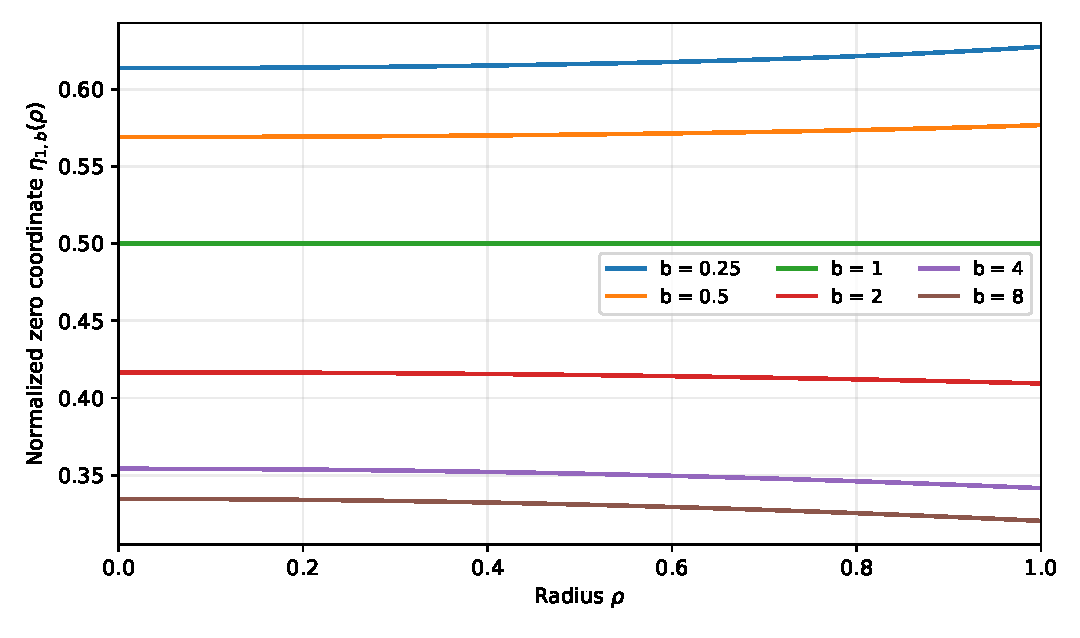
\includegraphics[width=0.94\linewidth]{figures/radial_motion.pdf}
\caption{The normalized-radius law at six inner orders. All strict signs
on the whole interval are proved in Theorem~\ref{thm:main}. The plotted
values use 256-node generalized Gauss--Laguerre quadrature and are
illustrative. Eighteen selected roots, including fractional inner
orders, have separate rational certificates.}
\label{fig:radial}
\end{figure}

\subsection{The whole upper-half-plane curve and the outer cutoff}
\begin{corollary}[A global parametrization and a sharp circle cutoff]
\label{cor:cutoff}
For every $b>0$, the entire upper-half-plane zero set of $\Imn F_b$ is
\begin{equation}\label{eq:globalcurve}
 z_b(y)=\frac1{m_b(y)-\ii y},\qquad y>0,
\end{equation}
where $m_b$ is the unique Cauchy mode associated with $Q_b$.
It is a simple analytic curve. If $b>1$, every circle of radius
$0<\rho<1/r_b$ has exactly one such upper-half-plane zero, and circles
of radius $\rho\ge1/r_b$ have none. For $b=1$ the cutoff is $2$.
For $b>1$ the normalized coordinate is strictly decreasing throughout
$0<\rho<1/r_b$, not only in the unit disk.
\end{corollary}
\begin{proof}
The parametrization follows from \eqref{eq:poissonidentity} and
Lemma~\ref{lem:mode}; it is injective because the inverse coordinate
$y$ is unique. Its derivative never vanishes: the derivative of
$m_b(y)-\ii y$ has imaginary part $-1$.
For $b>1$, $m_b>0$ and $m_b'>0$, so
\[
 R_b(y)=|z_b(y)|=(m_b(y)^2+y^2)^{-1/2}
\]
is strictly decreasing. Its limits are $1/r_b$ at $y\downarrow0$
and zero at infinity. This proves the circle count and cutoff.
Along the curve, $\eta_b(R_b(y))=m_b(y)$, giving the strict radial
sign on the whole interval. At $b=1$, $m_b=1/2$ and the same argument
has cutoff $2$. The limiting point $1/r_b$ lies on the excluded real
cut, not in the upper half-plane; it is not an omitted upper-arc zero.
\end{proof}

For $0<b<1$, the inverse coordinate $m_b(y)$ decreases, but this alone
does not determine the sign of $R_b'(y)$ outside the disk. The complete
inverse graph remains proved; a global circle-count assertion in this
range is deliberately not made.

\section{All odd central moments have a prescribed sign}
\label{sec:moments}
The reflection argument also gives a hierarchy of exact inequalities,
without introducing a smoothing kernel.

\begin{theorem}[Reflected skew inequalities]\label{thm:skew}
Let $U$ have density $2\Qw/\Wtot$ and mean $\mu_w$. Suppose $w$ is
nonconstant and nonincreasing. For every continuous strictly increasing
function $\varphi$ on $[0,1]$,
\begin{equation}\label{eq:skewphi}
 \E\big[(U-\mu_w)\varphi((U-\mu_w)^2)\big]>0.
\end{equation}
For a nonconstant nondecreasing weight the sign is negative.
For a constant weight it is zero. In particular, for every integer
$m\ge1$ the central moment $\E(U-\mu_w)^{2m+1}$ has the same sign.
\end{theorem}
\begin{proof}
Consider the nonincreasing case. We know $\mu_w<1/2$.
The mean identity is
\[
 \int_0^\infty v\Delta_{\mu_w}(v)\dd v
       =\int_0^1(u-\mu_w)\Qw(u)\dd u=0.
\]
Since $\Delta_{\mu_w}$ has a positive part, this forces a negative
part. Lemma~\ref{lem:reflection} supplies a unique crossing $v_0$.
Consequently
\[
 \int_0^\infty v\Delta_{\mu_w}(v)
             \bigl(\varphi(v^2)-\varphi(v_0^2)\bigr)\dd v>0.
\]
Division by $\Wtot/2$ proves \eqref{eq:skewphi}. Choosing
$\varphi(t)=t^m$ proves the moment assertion. Reflection handles the
opposite monotonicity, and symmetry handles a constant weight.
\end{proof}

\begin{corollary}[Explicit harmonic inequalities]\label{cor:harmonic}
For $b>0$ and every integer $m\ge1$, put $\mu_b=(1+2^{-b})/3$.
Then
\begin{equation}\label{eq:alloddharmonic}
 2\sum_{j=0}^{2m+1}\binom{2m+1}{j}(-\mu_b)^{2m+1-j}
       \frac{H_{j+1}^{(b)}}{(j+1)(j+2)}
\end{equation}
is positive for $b>1$, negative for $0<b<1$, and zero for $b=1$.
\end{corollary}
\begin{proof}
Expression~\eqref{eq:alloddharmonic} is the binomial expansion of
$\E(U_b-\mu_b)^{2m+1}$, using \eqref{eq:rawb}. Apply
Theorem~\ref{thm:skew} to $w_b$.
\end{proof}

The statement is a continuum theorem in $b$ and an all-order theorem
in $m$. Exact finite tests in the package are useful regression checks,
but are not its proof.

\begin{corollary}[An exponential version]\label{cor:mgf}
For every $\lambda>0$,
\[
 \E e^{\lambda(U_b-\mu_b)}-
 \E e^{-\lambda(U_b-\mu_b)}
\]
has the sign of $b-1$, with strictness for $b\ne1$.
\end{corollary}
\begin{proof}
The function $\varphi(t)=\sinh(\lambda\sqrt t)/\sqrt t$, defined at
zero by continuity, is strictly increasing on $[0,1]$: its power
series has a positive constant and strictly positive higher
coefficients. Equation~\eqref{eq:skewphi} gives the result, since
$(U-\mu)\varphi((U-\mu)^2)=\sinh(\lambda(U-\mu))$.
\end{proof}

\section{Radial expansions and a genuine curvature limitation}
\label{sec:expansion}
Write $M_j=\E(U-\mu)^j$ for the normalized Green law. These moments
are finite because the support is compact.

\begin{proposition}[Large-height mode expansion]\label{prop:mode-expansion}
For $\alpha>0$, put $p=\alpha+1$. As $y\to\infty$,
\begin{equation}\label{eq:studentexp}
 m_\alpha(y)=\mu-pM_3y^{-2}
   +\left(\frac{p(p+1)}2M_5-3p^2M_2M_3\right)y^{-4}
   +O(y^{-6}).
\end{equation}
No monotonicity assumption on $w$ is required for this expansion.
\end{proposition}
\begin{proof}
Let $V=U-\mu$, $d=m_\alpha(y)-\mu$, and $h=y^{-2}$. The stationary
equation is
\[
 0=\E\big[(V-d)(1+h(V-d)^2)^{-p}\big].
\]
At $h=0$ it has the simple solution $d=0$, with derivative $-1$ in
$d$. The analytic implicit-function theorem applies near $(0,0)$;
compact support makes the binomial expansion uniform there.
Expanding through $h^2$, using $d=O(h)$, gives
\[
 0=-d-pM_3h+3pM_2dh+\frac{p(p+1)}2M_5h^2+O(h^3).
\]
Solving successively for the coefficients of $h$ and $h^2$ yields
\eqref{eq:studentexp}.
\end{proof}

\begin{corollary}[Radial expansion through fourth order]
\label{cor:radialexp}
For the leading-index-one polylogarithm, with moments of $2Q_b$,
\begin{equation}\label{eq:etaexp}
 \eta_b(\rho)=\mu_b-2M_3\rho^2
 +\bigl[3M_5-(12M_2+2\mu_b^2)M_3\bigr]\rho^4+O_b(\rho^6).
\end{equation}
Let $U=H_2^{(b)}$, $V=H_3^{(b)}$, $W=H_4^{(b)}$. Then
\begin{equation}\label{eq:Kthird}
 -2M_3=\frac{UV}{3}-\frac W5-\frac{4U^3}{27}=K(1,b),
\end{equation}
where $K$ is the coefficient already recorded in the manuscript.
\end{corollary}
\begin{proof}
Take $\alpha=1$, so $p=2$, in \eqref{eq:studentexp}, and use
$y^{-2}=\rho^2/(1-\rho^2\eta_b(\rho)^2)
=\rho^2+\mu_b^2\rho^4+O(\rho^6)$.
The raw moments give
\[
 M_3=\frac W{10}-\frac{UV}{6}+\frac{2U^3}{27},
\]
which proves \eqref{eq:Kthird}.
\end{proof}

This proves the $a=1$ local sign by a conceptual positive-measure
argument and strengthens it globally. It is not a correction to the
existing formula: the existing formula agrees exactly.

\begin{proposition}[No universal radial-curvature sign]
\label{prop:curvaturecounter}
Let $s=\rho^2$. Although $\eta_b(\sqrt s)$ decreases for every $b>1$,
it is strictly concave near $s=0$ when $b=2$ and strictly convex there
when $b=4$. More precisely,
\begin{align}
 \eta_2(\rho)&=\frac5{12}-\frac1{144}\rho^2
                    -\frac{263}{777600}\rho^4+O(\rho^6),
                    \label{eq:b2exp}\\
 \eta_4(\rho)&=\frac{17}{48}-\frac{15893}{1244160}\rho^2
                    +\frac{504047}{3149280000}\rho^4+O(\rho^6).
                    \label{eq:b4exp}
\end{align}
In particular $s\mapsto\eta_2(\sqrt s)$ is not completely monotone
on any interval $(0,\varepsilon)$.
\end{proposition}
\begin{proof}
Substitute the rational moments from \eqref{eq:rawb} into
\eqref{eq:etaexp}. The two fourth-order coefficients are the exact
fractions displayed. The second $s$ derivative tends to twice that
coefficient, giving the strict signs near zero. Complete monotonicity
would require the second derivative to be nonnegative; the $b=2$
expansion excludes it.
\end{proof}

Thus a proposed upgrade from monotonicity to one fixed convexity or
complete-monotonicity class would be false. No such upgrade is alleged
to have been claimed by the inspected manuscript. The proposition is
a useful boundary for future conjecture formation.

\section{Hurwitz-shifted inner orders}
\label{sec:shift}
For real $\lambda>-1$, $b>0$, define
\begin{equation}\label{eq:shifted}
 F_b^{(\lambda)}(z)=\sum_{n\ge2}\frac{z^n}{n}
          \sum_{k=1}^{n-1}(k+\lambda)^{-b}.
\end{equation}
The corresponding admissible weight is
\begin{equation}\label{eq:shiftweight}
 w_{\lambda,b}(u)=\frac{u^\lambda(-\log u)^{b-1}}{\Gamma(b)}.
\end{equation}
Its mass is $(1+\lambda)^{-b}$; its Green transform and slit-plane
continuation are defined as before. The logarithmic derivative is
\begin{equation}\label{eq:shiftweightderivative}
 \frac{d}{du}\log w_{\lambda,b}(u)
 =\frac1u\left(\lambda-\frac{b-1}{-\log u}\right).
\end{equation}

\begin{theorem}[Two complete monotone sectors]\label{thm:shift}
Let $\eta_{\lambda,b}(\rho)$ denote the normalized angular zero for
$F_b^{(\lambda)}$. If $-1<\lambda\le0$ and $b\ge1$, excluding
$(\lambda,b)=(0,1)$, it is strictly decreasing on $0<\rho\le1$.
If $\lambda\ge0$ and $0<b\le1$, excluding the same point, it is
strictly increasing. At $(0,1)$ it is constant $1/2$.
In all these cases the analytic value at zero is
\begin{equation}\label{eq:shiftmean}
 \eta_{\lambda,b}(0)=\frac13\left[
        1+\left(\frac{1+\lambda}{2+\lambda}\right)^b\right].
\end{equation}
\end{theorem}
\begin{proof}
The gamma integral gives
$\int_0^1u^k w_{\lambda,b}(u)\dd u=(k+\lambda+1)^{-b}$,
so \eqref{eq:Fwcoeff} is exactly \eqref{eq:shifted}.
Equation~\eqref{eq:shiftweightderivative} gives strict decreasing or
increasing behavior in the indicated sectors. Apply
Theorem~\ref{thm:generalradial}. Formula~\eqref{eq:muw} gives
\eqref{eq:shiftmean}.
\end{proof}

The mixed sectors $\lambda>0,b>1$ and $-1<\lambda<0,0<b<1$ are not
covered by this monotone-curvature criterion. In those sectors the
weight can change its direction of monotonicity; no radial sign is
inferred merely from the sign of its first Taylor coefficient.

\section{Exact sums over all inner orders}
\label{sec:identities}
\subsection{A weight-generating transport identity}
\begin{theorem}[Order generation is a Hurwitz shift]\label{thm:generator}
For $|\tau|<1$ and $z\in\cut$,
\begin{equation}\label{eq:generator}
 \sum_{m=1}^{\infty}\tau^{m-1}F_m(z)=F_1^{(-\tau)}(z).
\end{equation}
For a complex shift on the right, the function is defined by its disk
series with denominators $k-\tau$ and its Green-integral continuation.
The convergence in \eqref{eq:generator} is locally uniform jointly in
$z$ and $\tau$.
\end{theorem}
\begin{proof}
In the disk, absolute convergence permits summation in the inner order:
\[
 \sum_{m\ge1}\frac{\tau^{m-1}}{k^m}=\frac1{k-\tau},\qquad k\ge1.
\]
This proves the coefficient identity. The same transport is visible
at the weight level:
\[
 \sum_{m\ge1}\tau^{m-1}\frac{(-\log u)^{m-1}}{(m-1)!}
                    =u^{-\tau}.
\]
To justify continuation and local uniformity, let $K\subset\cut$ be
compact and set
\[
 \delta_K=\min_{z\in K,\,0\le u\le1}|1-zu|>0,
 \qquad C_K=\frac{\max_{z\in K}|z|^2}{2\delta_K^2}.
\]
Each $Q_m$ has mass $1/2$, so \eqref{eq:Fw} gives
$|F_m(z)|\le C_K$, uniformly in the positive integer $m$. The
Weierstrass test proves the required convergence for $|\tau|\le q<1$.
The complex Green weight $u^{-\tau}$ is integrable since
$\Ren\tau<1$, and its integral is analytic in these parameters.
The identity theorem extends the disk equality to the slit plane.
\end{proof}

The same proof gives an explicit truncation bound:
\begin{equation}\label{eq:gentail}
 \left|\sum_{m>M}\tau^{m-1}F_m(z)\right|
       \le C_K\frac{|\tau|^M}{1-|\tau|}.
\end{equation}
Thus the all-order identity has a simple independently reproducible
analytic error contract.

\subsection{Half shifts and parity-separated identities}
Let
\[
 A(z)=\atanh\sqrt z.
\]
The individual square root need not be chosen globally in the slit
plane. In every formula below, only $A(z)^2$ and $\sqrt z\,A(z)$
appear. These are the single-valued analytic continuations from zero
of their power series, so the formulas are unambiguous at negative
real arguments as well.

\begin{proposition}[Two elementary shifted functions]\label{prop:halfshift}
On $\cut$,
\begin{align}
 F_1^{(-1/2)}(z)
       &=2A(z)^2-4\sqrt z\,A(z)-2\log(1-z),\label{eq:minusshift}\\
 F_1^{(1/2)}(z)
       &=2A(z)^2+2\log(1-z).\label{eq:plusshift}
\end{align}
\end{proposition}
\begin{proof}
Differentiating \eqref{eq:shifted} inside the disk gives
\begin{equation}\label{eq:shiftderivative}
 \frac d{dz}F_1^{(\lambda)}(z)
 =\frac1{1-z}\sum_{k\ge1}\frac{z^k}{k+\lambda}.
\end{equation}
The two inner sums at $\lambda=-1/2$ and $1/2$ are respectively
$2\sqrt z\,A(z)$ and $2(A(z)/\sqrt z-1)$.
With $z=r^2$, differentiation of the proposed expressions gives
$4r^2\atanh r/(1-r^2)$ and $4(\atanh r-r)/(1-r^2)$,
which agree with \eqref{eq:shiftderivative} after the chain rule.
Both expressions vanish at zero. Equality follows in the disk and
then by analytic continuation.
\end{proof}

\begin{theorem}[All odd and even inner orders]\label{thm:parity}
On $\cut$,
\begin{align}
 \sum_{j=0}^{\infty}4^{-j}F_{2j+1}(z)
       &=2A(z)^2-2\sqrt z\,A(z),\label{eq:oddidentity}\\
 \sum_{j=0}^{\infty}4^{-j}F_{2j+2}(z)
       &=-4\sqrt z\,A(z)-4\log(1-z).\label{eq:evenidentity}
\end{align}
After the first $J$ terms ($j=0,\ldots,J-1$), either tail has
absolute value at most $(4C_K/3)4^{-J}$ for $z\in K$.
\end{theorem}
\begin{proof}
Take the half-sum and the difference, respectively, of
\eqref{eq:generator} at $\tau=1/2$ and $\tau=-1/2$.
Insert \eqref{eq:minusshift}--\eqref{eq:plusshift}. The tail estimate
follows by the geometric series and $|F_m(z)|\le C_K$.
\end{proof}

\begin{corollary}[Four constant identities]\label{cor:constants}
In addition to \eqref{eq:introodd}--\eqref{eq:introeven},
\begin{align}
 \sum_{j\ge0}4^{-j}F_{2j+1}(1/4)
       &=\frac{\log^2 3-\log3}{2},\label{eq:quarterodd}\\
 \sum_{j\ge0}4^{-j}F_{2j+2}(1/4)
       &=8\log2-5\log3.\label{eq:quartereven}
\end{align}
At $z=-1$, either parity tail is at most $(2/3)4^{-J}$; at $z=1/4$
it is at most $(2/27)4^{-J}$.
\end{corollary}
\begin{proof}
At $z=-1$, take $\sqrt z=\ii$, so $A(z)=\ii\pi/4$.
At $z=1/4$, $\sqrt z=1/2$ and $A(z)=\log3/2$.
Substitution gives the identities. The constants in the tail bound
are $C_{\{-1\}}=1/2$ and $C_{\{1/4\}}=1/18$.
\end{proof}

These identities organize an infinite family of different weights into
a closed function. They do not express each separate $F_m(-1)$ in
an elementary basis, and hence do not settle finite-weight period
independence or the S6/S8 questions.

\subsection{Positive integer shifts reduce to ordinary polylogarithms}
For completeness, positive integral shifts give another exact family
that is useful for checking implementations. Put $L=\Li_1(z)=-\log(1-z)$
and $P_j(z)=\sum_{k=1}^jz^k/k$.

\begin{proposition}[Finite reduction for integral shifts]\label{prop:integer-shift}
For every integer $m\ge1$,
\begin{equation}\label{eq:integer-shift}
 F_1^{(m)}(z)=\frac12L^2+\Li_2(z)-\frac Lm
       +\sum_{j=1}^{m-1}\frac{z^{-j}}j\bigl(P_j(z)-L\bigr).
\end{equation}
Every apparent pole at zero in the finite sum is removable.
\end{proposition}
\begin{proof}
Since $P_j-L=-\sum_{k\ge j+1}z^k/k$, each summand is analytic at
zero. The coefficient of $z^n$, $n\ge1$, on the right is
\[
 \frac{H_{n-1}}n+\frac1{n^2}-\frac1{mn}
                   -\sum_{j=1}^{m-1}\frac1{j(n+j)}
 =\frac{H_{n+m-1}-H_m}{n}.
\]
Use $1/(j(n+j))=(1/j-1/(n+j))/n$ for the simplification.
This is exactly the coefficient in \eqref{eq:shifted}; the constant
terms vanish. Analytic continuation proves the formula on the slit
plane.
\end{proof}

\section{Verification, rational certificates, and numerical illustration}
\label{sec:verification}
\subsection{What is proved by which evidence}
All continuum statements above are proved by the analytic arguments.
The computational package has three different roles. Exact finite
coefficient and moment tests catch transcription errors. Rational
intervals with an infinite-series tail bound certify selected numerical
roots. Floating-point quadrature illustrates the geometry and checks
against a different evaluation formula; it is not an interval proof.
The three kinds of evidence are reported separately.

The executed standard-library verifier produced 180 exact odd-moment
sign checks (integer $b=1,\ldots,12$, odd orders $3,5,\ldots,31$),
768 coefficient equalities for the half-shift identities, 960 coefficient
equalities for positive integer shifts, and 30 checks of
$K(1,b)=-2M_3$. Their total is 1,938. A separate SymPy script checks
five symbolic identities, including the universal fourth-order radial
coefficient in five independent raw moments. These are finite replays,
not proof-assistant formalizations.

\subsection{A rational certificate for selected angular zeros}
Fix rational $0<\rho<1$ and rational $0<\eta<1$. Put
$x=\rho^2\eta$ and $s=\rho^2$. Although the imaginary coordinate of
$z=x+\ii\sqrt{s-x^2}$ need not be rational, the normalized powers
\[
 P_0=0,\quad P_1=1,\quad P_n=2xP_{n-1}-sP_{n-2}
\]
are rational, and equal $\Imn(z^n)/\Imn z$. Thus
\begin{equation}\label{eq:certificate-series}
 J=\frac{\Imn F_b(z)}{\Imn z}
      =\sum_{n\ge2}\frac{H_{n-1}^{(b)}}nP_n.
\end{equation}
The elementary inequality $|\sin(n\theta)|\le n\sin\theta$ for
$0<\theta<\pi$ gives $|P_n|\le n\rho^{n-1}$.
Since $H_{n-1}^{(b)}\le n-1$ for all $b>0$, the tail after outer
index $N$ is bounded by the rational number
\begin{equation}\label{eq:rationaltail}
 B_N(\rho)=\rho^N\left(\frac N{1-\rho}
                       +\frac{\rho}{(1-\rho)^2}\right).
\end{equation}

For positive integral $b$, every retained coefficient is rational.
For $b=1/2$ and $1/4$, the verifier encloses each $k^{-b}$ by rational
numbers with denominator $D=10^{60}$, using integer square roots only.
More generally, if $b=p/q$ and $q$ is a power of two, it finds $a$ with
\[
 a^q k^p\le D^q<(a+1)^q k^p,
\]
which proves $a/D\le k^{-b}<(a+1)/D$. Harmonic partial sums are then
propagated as rational intervals, with multiplication signs handled
exactly. No floating-point approximation is used to choose a sign in
the verifier.

For each proposed pair $\eta_-<\eta_+$, the script proves that the
upper enclosure of the truncated series at $\eta_-$ plus $B_N$ is
negative, and that the lower enclosure at $\eta_+$ minus $B_N$ is
positive. Lemma~\ref{lem:angular} then places the unique root strictly
between them. The executed suite certifies 18 brackets at
\[
 b\in\{1/4,1/2,2,3,4,8\},\qquad
 \rho\in\{1/4,1/2,3/4\},\qquad N=192.
\]
Every bracket has width $3\cdot10^{-10}$. All endpoints, exact sign
margins, and rational tail bounds are in the JSON receipt. For example,
\begin{align}
 \frac{829818637}{2000000000}
 &<\eta_2(1/2)<\frac{1037273297}{2500000000},
       \label{eq:examplebracket}\\
 0.4149093185&<\eta_2(1/2)<0.4149093188.\notag
\end{align}
The decimal line is just the terminating decimal form of the rational
endpoints; it does not introduce a separate rounding assertion.

\subsection{Independent floating-point diagnostics}
For numerical illustration we use the single-integral identity
\begin{equation}\label{eq:numericalintegral}
 F_b(z)=\int_0^1 w_b(t)
 \frac{\log(1-tz)/t-\log(1-z)}{1-t}\dd t.
\end{equation}
It follows by integrating $F_b'(z)=\Li_b(z)/(1-z)$ from zero and
inserting the gamma integral for $\Li_b$. Equivalently, one may
expand the two logarithms and compare the coefficients directly.
The apparent $t=0$ and $t=1$ singularities of the kernel are removable
for fixed slit-plane $z$.

With $t=e^{-T}$, generalized Gauss--Laguerre quadrature applies to the
weight $e^{-T}T^{b-1}/\Gamma(b)$. The diagnostic script uses 256 nodes,
compares with 128 nodes, and also compares 24 values against an
independent 70-digit, 1,024-term direct double-polylogarithm series
strictly inside the disk. The maximum observed absolute discrepancy
against that series was $3.38\cdot10^{-12}$. The script checks the
predicted monotonic direction on a 606-point grid, including the
analytic $\rho=0$ values. This finite grid has no role in proving
Theorem~\ref{thm:main}.

\begin{table}[tbp]
\centering
\small
\begin{tabular}{@{}rrrrrr@{}}
\toprule
$b$ & $\eta_b(0)$ & $\eta_b(1/4)$ & $\eta_b(1/2)$
    & $\eta_b(3/4)$ & $\eta_b(1)$\\
\midrule
$1/4$&0.6136321384&0.6142725544&0.6163248312&0.6202820025&0.6275145907\\
$1/2$&0.5690355937&0.5694172146&0.5706248931&0.5728838669&0.5767481557\\
$1$&0.5000000000&0.5000000000&0.5000000000&0.5000000000&0.5000000000\\
$2$&0.4166666667&0.4162313162&0.4149093186&0.4126523072&0.4093780509\\
$4$&0.3541666667&0.3533689224&0.3509838169&0.3470392575&0.3415922469\\
$8$&0.3346354167&0.3337176588&0.3309859468&0.3265081195&0.3204054688\\
\bottomrule
\end{tabular}
\caption{Illustrative quadrature values. The separate rational receipts
certify selected interior-radius brackets, not every printed digit of
every entry. At $b=1$ the value is exactly $1/2$.}
\label{tab:values}
\end{table}

\subsection{Reproduction and artifact contract}
The package is additive and does not change the repository remotely.
From its root, use fresh output directories:
\begin{verbatim}
python verification/verify_exact.py --output-dir /tmp/polylog-exact
python verification/verify_symbolic.py --output-dir /tmp/polylog-symbolic
python verification/verify_numeric.py --output-dir /tmp/polylog-numeric \
  --figures-dir /tmp/polylog-figures
pdflatex -interaction=nonstopmode -halt-on-error article.tex
pdflatex -interaction=nonstopmode -halt-on-error article.tex
\end{verbatim}
The exact verifier uses only the Python standard library. The symbolic
script uses SymPy; numerical diagnostics use NumPy, SciPy, mpmath, and
Matplotlib. Each script refuses to overwrite its own named result file,
so replaying into a new directory preserves received evidence. The
included receipts record what was actually executed in this session.
No checksum-normalization workflow is required.

\section{Audit findings and integration guidance}
\label{sec:audit}
\subsection{A status correction, not a correction to a valid formula}
In the inspected local-radius section, the whole-radius $a=1$ branch
is still framed as a conjectural extension of the local result.
After this article is reviewed, the appropriate update is narrow:
replace that branch's open status by Theorem~\ref{thm:main}, and retain
the distinction between it and all larger outer orders. The existing
local coefficient agrees with \eqref{eq:Kthird}; its proof is not
invalidated. The earlier Bernstein calculation remains useful evidence
and historical context.

The section on Cartesian motion proves an outward abscissa law and
explicitly distinguishes it from normalized-radius motion~\cite{repo-cartesian}.
That distinction is correct. The present proof fills one part of the
remaining normalized question by \eqref{eq:etasderivative}; it does
not reinterpret the Cartesian theorem as something stronger.

\subsection{Two small notation repairs in the transport proof}
In the inspected \src{05-real-positive-kernel.tex}, the proof of the
Hurwitz--polylogarithm transport theorem says to use the Hurwitz formula
``with $q=n$'', although its argument is named $x$; this should read
``with $x=n$''. The same proof invokes ``boundedness of $h$'', although
the regularized kernel in that argument is $q(t)$; it should read
``boundedness of $q$''~\cite{repo-positive}. These are local notation
repairs, not refutations of the transport identity. They are not
asserted to be first discoveries and may already be tracked in
incoming work. The integration notes keep them separate from the
new mathematical claim.

\subsection{Why the same proof does not automatically cover larger outer orders}
For integer $a\ge2$, the source signed kernels satisfy
$\kappa_{a,b}'(u)=-\kappa_{a-1,b}(u)/u$.
If $Q_{a,b}(u)=\int_u^1\kappa_{a,b}(v)\dd v$, then
\begin{equation}\label{eq:highercurvature}
 Q_{a,b}''(u)=\frac{\kappa_{a-1,b}(u)}u.
\end{equation}
The right side changes sign. Thus $Q_{a,b}$ is not generally concave,
and Lemma~\ref{lem:mode} cannot simply be invoked with that density.
This identifies the hypothesis that fails in a tempting extension;
it is not a claim that the higher-index conjecture is false or
inaccessible. Other representations or a more flexible sign criterion
may still prove it.

\subsection{What this audit does not certify}
The audit is local to the named analytic material and the displayed
formulas. It does not certify the entire 379-page manuscript, all
historical reports, all incoming ZIP members, period independence,
or the correctness of unrelated analytic continuations. The article
has not been independently refereed. All source-linked assertions can
be checked against the recorded paths and pin; the new theorems have
complete proofs here rather than relying on numerical plausibility.

\section{Further research questions}
\label{sec:future}
\begin{enumerate}[leftmargin=*,itemsep=7pt]
\item \textbf{Higher outer orders.} Find a replacement for strict
concavity in the proof of Lemma~\ref{lem:mode}, compatible with the
single change of curvature in \eqref{eq:highercurvature}. A useful
intermediate target is a signed reflected-difference criterion that
still controls the implicit radial denominator and numerator
separately. Any progress should be compared with the latest incoming
large-order and all-depth results before assigning an open range.

\item \textbf{The subunit-inner-order curve outside the disk.}
For $0<b<1$, determine the sign changes of
$m_b(y)m_b'(y)+y$, which controls $R_b'(y)$ in
Corollary~\ref{cor:cutoff}. Does each circle meet the upper imaginary-zero
curve at most once, or can the inverse-mode graph produce radial
turning? The complete parametrization \eqref{eq:globalcurve} reduces
the problem to one scalar analytic function, but its sign is not
settled here.

\item \textbf{Sharp quantitative motion bounds.} Formula
\eqref{eq:etasderivative} proves strictness but does not give a simple
optimal lower bound for $|\eta_b'(\rho)|$. Bound the reflected crossing
$v_0$ and the two sign-definite integrals to obtain uniform estimates
on compact $(b,\rho)$ ranges, especially as $b\to1$ or $\rho\to1$.

\item \textbf{Complete curvature classification.} The exact fourth-order
coefficient
$3M_5-(12M_2+2\mu_b^2)M_3$ is negative at $b=2$ and positive at $b=4$.
Determine all its zeros for $b>1$, with rigorous enclosures, and study
whether they govern changes in the full radial curvature rather than
only near the origin. This question must not be confused with the
already proved first-derivative sign.

\item \textbf{The mixed shifted sectors.} Classify normalized-radius
motion for $\lambda>0,b>1$ and $-1<\lambda<0,0<b<1$. In these regions
\eqref{eq:shiftweightderivative} has a zero. A natural task is to
classify the number of reflected sign changes and the possible
number of radial turning points before attempting a global phase
diagram.

\item \textbf{More general smoothing kernels.} The proof of
\eqref{eq:It-sign} uses that the logarithmic scale derivative of the
positive stationary weight is increasing in the reflection distance.
Formulate a maximal kernel class with that property. Gaussian kernels
are a natural comparison; kernels whose scale score changes direction
may expose necessary rather than merely sufficient shape hypotheses.

\item \textbf{Rational shifts and finite-weight consequences.}
The order-generating identity \eqref{eq:generator} converts rational
values of $\tau$ to rational shifts. Determine which such shifts have
useful logarithmic or cyclotomic descriptions and whether their
coefficient extractions yield new finite-weight identities. Infinite
weight sums alone do not prove the S6 or S8 reductions.

\item \textbf{Formalization and certified continuation.}
The finite rational root verifier is already suitable for independent
reimplementation. Formalize the Green regularity lemma, the signed
zero-mass comparison, the reflected single crossing, and the implicit
radial derivative as separate components. Extend the rational
certificates toward $\rho=1$ using a rigorously accelerated series or
positive-kernel quadrature, rather than labeling ordinary quadrature
as certified.
\end{enumerate}

\section{Conclusion}
The leading-index-one normalized-radius conjecture is resolved by a
shape theorem for a positive Green density. The decisive information
is not simply positivity or uniqueness of an angular zero: it is the
ordered sign change of a reflected density, followed by a careful
change from inverse-height differentiation to radial differentiation.
This proves all three inner-order regimes on the full disk, gives a
larger global domain when $b\ge1$, and supplies both moment inequalities
and exact all-order identities. The proof also exposes a real limit of
stronger conjectures through opposite local curvature signs. The
remaining higher-index, mixed-shift, and finite-weight arithmetic
questions are separated from these proved statements rather than
being hidden behind a numerical residual.

\clearpage
\begin{thebibliography}{20}
\bibitem{repo-local}
ProveIt Contributors, \emph{A proved local part of the normalized-radius
conjecture}, in \emph{Polylogarithms and their Arithmetic Bridges},
\src{Analysis/Polylogarithms/docs/manuscript/chapters/05-real-local-radius.tex},
inspected at commit \repocommit, 10 October 2026.
\url{https://github.com/VladimirReshetnikov/ProveIt/blob/1539f353af88bdfd63292bb970ac8f585b15794d/Analysis/Polylogarithms/docs/manuscript/chapters/05-real-local-radius.tex}.

\bibitem{repo-signed}
ProveIt Contributors, \emph{A signed-kernel representation; the unique zero
on the upper semicircle},
\src{Analysis/Polylogarithms/docs/manuscript/chapters/05-signed-kernels.tex},
repository source consulted 10 October 2026.
\url{https://github.com/VladimirReshetnikov/ProveIt/tree/main/Analysis/Polylogarithms/docs/manuscript}.

\bibitem{repo-readme}
ProveIt Contributors, \emph{Polylogarithms and their Arithmetic Bridges:
manuscript README}, consulted 10 October 2026; inspected blob
\src{8c96411966c6711b90ed54a86dfbeb2963b58190}.
\url{https://github.com/VladimirReshetnikov/ProveIt/blob/main/Analysis/Polylogarithms/docs/manuscript/README.md}.

\bibitem{repo-cartesian}
ProveIt Contributors, \emph{Cartesian motion of the complete real-order
zero arc}, \src{chapters/05-real-cartesian-motion.tex}, consulted
10 October 2026; inspected blob
\src{0deb9bb54adaef8783d4e0e7ce43d426643450a0}.

\bibitem{repo-positive}
ProveIt Contributors, \emph{A positive two-variable representation at all
positive orders}, \src{chapters/05-real-positive-kernel.tex}, consulted
10 October 2026; inspected blob
\src{044d3825b90dce437ac9007733e6447cf9563098}.

\bibitem{ibragimov}
I.~A. Ibragimov, On the composition of unimodal distributions,
\emph{Theory of Probability and its Applications} \textbf{1} (1956),
255--260. \url{https://doi.org/10.1137/1101021}.
Primary journal record and abstract:
\url{https://www.mathnet.ru/eng/tvp5002}.

\bibitem{liu-pego}
J.-G. Liu and R.~L. Pego, On generating functions of Hausdorff moment
sequences, \emph{Transactions of the American Mathematical Society}
\textbf{368} (2016), 8499--8518.
\url{https://doi.org/10.1090/tran/6618}.
Consulted arXiv version 4, 12 November 2025, including corrigendum:
\url{https://arxiv.org/abs/1401.8052v4}.

\bibitem{dlmf}
F.~W.~J. Olver et al., eds., \emph{NIST Digital Library of Mathematical
Functions}, Section 25.12, Polylogarithms; consulted 10 October 2026.
\url{https://dlmf.nist.gov/25.12}.
\end{thebibliography}
\end{document}
